\documentclass[10pt]{article}
\usepackage[margin=0.9in]{geometry}
\usepackage{amsmath,amssymb,booktabs,graphicx,microtype,xcolor,hyperref,caption,subcaption,enumitem}
\usepackage[T1]{fontenc}
\hypersetup{colorlinks=true,linkcolor=blue!50!black,citecolor=blue!50!black,urlcolor=blue!50!black}
\setlist{nosep,leftmargin=*}
% AUTO-GENERATED by bench/claims.py from results/ -- do not edit
\makeatletter
\newcommand{\claim}[1]{\@ifundefined{claim@#1}{\textbf{??#1??}}{\csname claim@#1\endcsname}}
\expandafter\def\csname claim@M1_PL_d5_p003_PM\endcsname{3.62e-03}  % [sim (Monte Carlo, Stim)] results/M1/pl/pl_d5_p0.003.json
\expandafter\def\csname claim@M1_PL_d5_p003_UF\endcsname{4.04e-03}  % [sim (Monte Carlo, Stim)] results/M1/pl/pl_d5_p0.003.json
\expandafter\def\csname claim@M1_PL_d7_p003_PM\endcsname{1.51e-03}  % [sim (Monte Carlo, Stim)] results/M1/pl/pl_d7_p0.003.json
\expandafter\def\csname claim@M1_PL_d7_p003_UF\endcsname{1.92e-03}  % [sim (Monte Carlo, Stim)] results/M1/pl/pl_d7_p0.003.json
\expandafter\def\csname claim@M1_PL_d9_p003_PM\endcsname{5.58e-04}  % [sim (Monte Carlo, Stim)] results/M1/pl/pl_d9_p0.003.json
\expandafter\def\csname claim@M1_PL_d9_p003_UF\endcsname{7.93e-04}  % [sim (Monte Carlo, Stim)] results/M1/pl/pl_d9_p0.003.json
\expandafter\def\csname claim@M1_p99_d5_p003_PM_us\endcsname{3.25}  % [CPU measurement (1 thread)] results/M1/latency.json
\expandafter\def\csname claim@M1_p99_d5_p003_UF_us\endcsname{2.92}  % [CPU measurement (1 thread)] results/M1/latency.json
\expandafter\def\csname claim@M1_p99_d7_p003_PM_us\endcsname{7.54}  % [CPU measurement (1 thread)] results/M1/latency.json
\expandafter\def\csname claim@M1_p99_d7_p003_UF_us\endcsname{7.21}  % [CPU measurement (1 thread)] results/M1/latency.json
\expandafter\def\csname claim@M1_thr_PM_7_9\endcsname{0.0078}  % [sim (Monte Carlo, curve crossing)] results/M1/summary.json
\expandafter\def\csname claim@M1_thr_UF_7_9\endcsname{0.0072}  % [sim (Monte Carlo, curve crossing)] results/M1/summary.json
\makeatother

\newcommand{\stage}[1]{\textsf{\small[#1]}}
\graphicspath{{../results/}}

\title{QShield-X: A Formally Checked, FPGA-Targeted Union-Find Decoder for the Surface Code,\\
with a WebAssembly Runtime and a V8 Code-Generation Fix}
\author{QShield-X project}
\date{Draft --- all numbers are generated from \texttt{results/} by \texttt{bench/claims.py}}

\begin{document}
\maketitle

\begin{abstract}
We ask whether hardware--software co-design with formally checked execution protocols gives a better
logical-error / latency / resource trade-off than a fixed software decoder for rotated surface-code memory
experiments under circuit-level depolarizing noise. We build \emph{QSX-UF}, a union-find decoder whose
semantics are made evaluation-order independent so that a fully parallel SystemVerilog implementation and a
sequential C++ golden model agree bit-for-bit, including the correction bitmap and the cycle count. The RTL
agrees with the golden model on \claim{M2_cosim_total} co-simulated syndromes with \claim{M2_cosim_mm} mismatches.
Shell properties (backpressure, round tags, no invalid result presented as valid, atomic reconfiguration,
AXI-Stream compliance) are proven by k-induction; the host/accelerator/fallback protocol is model-checked in
TLA+, where TLC found a liveness bug that we fixed; and Z3 proves one-step equivalence of the real core against an
independent reference. On a Lattice ECP5-85F (open toolchain, post-place-and-route, no board), the decoder
reaches a p99 latency of \claim{M2_hw_p99_ns_d5}\,ns per $d$-round block at $d=5$ \stage{sim cycles / PnR
Fmax}, versus \claim{M1_p99_d5_p003_PM_us}\,\textmu s for PyMatching on one CPU core \stage{CPU}, at the cost
of a \claim{M1_ratio_d5_p003}$\times$ higher logical error rate \stage{Monte Carlo}. The answer to the
central question is therefore \emph{mixed}: large latency gains with bounded, verified behaviour, paid for in
accuracy and in FPGA area that grows quickly with distance. We also report a Wasm SIMD study, an upstreamable V8
arm64 code-generation fix found while profiling the decoder, adaptive and learned decoding under noise
shifts, and a federated-learning simulation with differential privacy.
\end{abstract}

\section{Introduction}
Fault-tolerant quantum computing needs a classical decoder that keeps up with the syndrome stream.
For superconducting devices one round of stabilizer measurements takes on the order of a microsecond, so
a decoder that falls behind builds up a backlog that eventually stalls the logical computation
\cite{fowler2012,google2025below}. Minimum-weight perfect matching (MWPM) is accurate and fast in software
\cite{higgott2022pymatching,higgott2023sparse}, but its data structures (priority queues, alternating trees)
are awkward to bound in hardware. Union-find (UF) decoding \cite{delfosse2021uf} uses small integer state and
local operations and is the basis of several hardware decoders \cite{das2022afs,liyanage2023helios,barber2023realtime}.

A decoder in a control stack is also a \emph{protocol participant}: it receives frames under backpressure,
returns results tagged with the measurement round they belong to, may time out, may be reconfigured, and
may be bypassed by a software fallback. These behaviours are where integration bugs live, and none of them
is captured by a logical-error-rate plot. QShield-X treats them as first-class, checkable properties.

\paragraph{Question.} Can hardware--software co-design with formally checked execution protocols deliver a
better logical-error / latency / resource trade-off than a fixed software-only decoder, for rotated
surface-code memory experiments with $d\in\{3,5,7,9\}$ under uniform circuit-level depolarizing noise?

\paragraph{Contributions.}
\begin{itemize}
\item \textbf{QSX-UF}, a Jacobi-synchronous union-find decoder with a canonical spanning forest, defined so
  that parallel RTL and sequential C++ are bit- and cycle-exact (\S\ref{sec:alg}); weighted (3-bit) and
  unweighted variants; P\textsubscript{L} measured against PyMatching with exact binomial confidence
  intervals (\S\ref{sec:eval-pl}).
\item A parameterised SystemVerilog microarchitecture (AXI-Stream shell, commit-on-last frame FIFO, atomic
  configuration, watchdog, LANES-wide scans) with Verilator co-simulation and an open-source ECP5 flow
  (\S\ref{sec:uarch}, \S\ref{sec:eval-hw}).
\item Formal verification at three levels with stated bounds: SVA/SymbiYosys k-induction on the RTL, TLA+/TLC on
  the host protocol (a real counterexample and its fix), and Z3 step equivalence of the core
  (\S\ref{sec:verif}).
\item A native/Wasm-scalar/Wasm-SIMD runtime study, and an in-tree V8 patch with unittests and an mjsunit
  test that removes a redundant compare/set from \texttt{v128.any\_true}-guarded branches on arm64
  (\S\ref{sec:wasm}).
\item Extensions: GNN decoding and an adaptive policy under noise shifts; federated training with DP-SGD and
  simulated secure aggregation; signed and encrypted experiment artefacts (\S\ref{sec:ext}).
\end{itemize}
Every number in this paper is generated from a result file that records the git commit, tool versions, seed
and configuration. Hardware numbers carry their evidence stage in brackets: \stage{sim} (Verilator or the
cycle-exact model), \stage{synth} (Yosys), \stage{PnR} (nextpnr). No number comes from a physical FPGA board,
and none of this is an ASIC result.

\section{Background}
\paragraph{Surface-code memory.} We use Stim's \texttt{surface\_code:rotated\_memory\_z} circuits
\cite{gidney2021stim} with $d$ rounds and the same probability $p$ for two-qubit depolarization after
Cliffords, data depolarization before each round, measurement flips, and reset flips. A shot fails if the
decoder's prediction of the logical observable differs from the true flip; P\textsubscript{L} is the failure
probability per $d$-round block. The decoder input is the set of \emph{detection events} (defects); the
decoding graph comes from the detector error model with \texttt{decompose\_errors}, parallel edges merged,
and one virtual boundary vertex.

\paragraph{Union-find decoding.} UF \cite{delfosse2021uf} grows clusters around defects in half-edge steps,
merges clusters that touch, stops growing a cluster once it has even parity or touches the boundary, and then
\emph{peels} a spanning forest of each cluster to obtain a correction. Weighted UF \cite{huang2020weighted}
grows edges at speeds proportional to their log-likelihood weight. The original algorithm grows the
smallest odd cluster first; its outcome depends on processing order, which is what QSX-UF removes.

\section{QSX-UF: an order-independent union-find}\label{sec:alg}
QSX-UF (DECISIONS D1) keeps an integer support $s_e\in[0,t_e]$ per edge, with growth threshold
$t_e\in[1,15]$. An edge is grown iff $s_e=t_e$. Clusters are connected components of grown non-boundary
edges. A vertex is \emph{active} iff its cluster has odd parity and no grown boundary edge. One growth round
is a synchronous (Jacobi) update $s_e\leftarrow\min(t_e, s_e+a_u+a_v)$ using activities from before the
round. Rounds repeat while any vertex is active, up to \texttt{max\_rounds}; on expiry the status is
\texttt{TIMEOUT} and the correction is all-zero. The spanning forest is canonical: the root of a cluster is
the boundary if the cluster touches it, else its minimum-index vertex; BFS distances are computed in
parallel, and each vertex picks the \emph{lowest-index} grown incident edge towards distance $-1$. Peeling
proceeds in decreasing distance. Since every step is a function of the previous state only, a parallel
implementation and a sequential one produce identical supports, forests and corrections.

Thresholds are quantised log-likelihood weights, $t_e=\mathrm{clamp}(\mathrm{round}(5\,w_e/\mathrm{median}(w)),1,7)$
(\texttt{q5}, 3-bit counters, chosen by a pilot study, DECISIONS D5), or $t_e=2$ for the minimal-area
unweighted variant.

\section{Microarchitecture}\label{sec:uarch}
\paragraph{Core.} The edge fabric holds all $E$ support counters and updates them in one cycle per growth
round. The vertex fabric holds per-vertex labels and computes cluster labels by min-label propagation over
grown edges (balanced min trees), one hop per cycle until convergence. It also holds BFS distances, one-hot
parent-edge selection, and self-timed peeling, where a vertex fires once all its children are done. Cluster
parity, boundary flags and the activity broadcast are computed by \emph{LANES} scans that process LANES
vertices per cycle, so the compute-unit parameter trades area for $2\lceil V/\text{LANES}\rceil$ cycles per round.
The FSM is \texttt{IDLE}$\to$\texttt{LABEL*}$\to$\texttt{PAR}$\to$\texttt{ACT}$\to$\texttt{CHK}$\to$(\texttt{GROW}$\to\cdots$)$\to$\texttt{DIST*}$\to$\texttt{PEH}$\to$\texttt{PEEL*}$\to$\texttt{DONE}.
An optional pipeline register (PIPE) adds one cycle per LABEL and DIST step to shorten the critical path.
Safety mechanisms: the \texttt{max\_rounds} timeout, a \texttt{cycle\_budget} watchdog, fail-closed
peeling, and zeroed outputs for any non-OK status.

\paragraph{Shell.} Input frames are a header carrying a 16-bit round tag plus $\lceil V/32\rceil$ syndrome beats
over AXI-Stream. They enter a BRAM ring of NBUF slots that commits a frame only on its last beat and
de-asserts \texttt{tready} when full. A dispatcher starts the core only when the configuration is valid and
closed. The egress emits a header (magic, status, observable, tag) and optionally the $E$-bit correction.
Malformed frames are answered in order with \texttt{FRAME\_ERROR}. Configuration is an atomic
BEGIN/WRITE/COMMIT session: COMMIT validates only if every threshold word was written and every value is
in range; otherwise frames are answered \texttt{CFG\_INVALID} and never decoded.

\section{Verification}\label{sec:verif}
\subsection{Co-simulation}
Verilator models of the core and of the full shell are compared, per syndrome, against the C++ golden
model \texttt{qsx::HwModel} on status, round count, observable, the full correction bitmap and the cycle
count. Inputs are random syndromes over densities $0$--$0.9$ and Stim-sampled syndromes at
$p\in\{0.001,0.003,0.006,0.01\}$. The shell tests add input gaps, output backpressure, malformed frames and
mid-stream reconfiguration, including deliberately incomplete sessions (Table~\ref{tab:cosim}).

\subsection{SVA and SymbiYosys}
Table~\ref{tab:formal} lists the properties and their results. The shell harness replaces the core by an
abstract stub that may take any latency and return any status and correction, subject only to the core's
interface guarantees. Those guarantees are themselves proven on the real core ($d=3$). The shell proofs
therefore hold for every core behaviour. A bounded check of the composition with the real core
complements them.

\subsection{TLA+ protocol model}
\texttt{QSXProtocol.tla} models a host that submits rounds to a $K$-deep accelerator queue, receives
tagged responses, filters stale ones, checks status, falls back to software after a deadline or an error,
and commits rounds in order. It also models reconfiguration sessions that the accelerator may only accept when
empty. The accelerator gets \emph{no} fairness: it may stall or lose requests forever. Safety:
\textsf{NoDoubleCommit}, \textsf{NoSkip}, \textsf{ExclusiveSource} (hardware xor software),
\textsf{NoInvalidCommit}, \textsf{NoOverflow}. Liveness: every round is eventually committed, under weak
fairness of host, timer, fallback and session close. The first version violated liveness: requests that had
timed out stayed in a stalled accelerator, filled its queue and blocked every later submission. We fixed it
with a submission deadline that bypasses the accelerator. Mutations that remove the stale filter or the
status check each violate safety, which shows the invariants are not vacuous.

\subsection{Z3 step equivalence}
Yosys exports the flattened core as an SMT-LIB transition relation. For \emph{all} register and input values,
reachable or not, Z3 \cite{demoura2008z3} proves that one clock step of each FSM phase (LABEL, GROW, DIST, PEH)
equals a reference built independently from the graph file. This also validates the table generator. A
mutated reference (highest-index parent) is SAT, which guards against vacuity.

% AUTO-GENERATED by bench/claims_ext.py -- do not edit
\begin{table}[t]\centering\footnotesize
\caption{Formal verification jobs (\texttt{make formal}). ``prove'' = k-induction (unbounded); ``bmc'' = bounded to the stated depth; TLC explores the full state space of the stated model constants.}
\label{tab:formal}
\begin{tabular}{llllr}\toprule job & tool & bound & result & s \\ \midrule
\claim{M3F_0_job} & \claim{M3F_0_tool} & \claim{M3F_0_bound} & \claim{M3F_0_status} & \claim{M3F_0_sec} \\
\claim{M3F_1_job} & \claim{M3F_1_tool} & \claim{M3F_1_bound} & \claim{M3F_1_status} & \claim{M3F_1_sec} \\
\claim{M3F_2_job} & \claim{M3F_2_tool} & \claim{M3F_2_bound} & \claim{M3F_2_status} & \claim{M3F_2_sec} \\
\claim{M3F_3_job} & \claim{M3F_3_tool} & \claim{M3F_3_bound} & \claim{M3F_3_status} & \claim{M3F_3_sec} \\
\claim{M3F_4_job} & \claim{M3F_4_tool} & \claim{M3F_4_bound} & \claim{M3F_4_status} & \claim{M3F_4_sec} \\
\claim{M3F_5_job} & \claim{M3F_5_tool} & \claim{M3F_5_bound} & \claim{M3F_5_status} & \claim{M3F_5_sec} \\
\claim{M3F_6_job} & \claim{M3F_6_tool} & \claim{M3F_6_bound} & \claim{M3F_6_status} & \claim{M3F_6_sec} \\
\claim{M3F_7_job} & \claim{M3F_7_tool} & \claim{M3F_7_bound} & \claim{M3F_7_status} & \claim{M3F_7_sec} \\
\claim{M3F_8_job} & \claim{M3F_8_tool} & \claim{M3F_8_bound} & \claim{M3F_8_status} & \claim{M3F_8_sec} \\
\claim{M3F_9_job} & \claim{M3F_9_tool} & \claim{M3F_9_bound} & \claim{M3F_9_status} & \claim{M3F_9_sec} \\
\claim{M3F_10_job} & \claim{M3F_10_tool} & \claim{M3F_10_bound} & \claim{M3F_10_status} & \claim{M3F_10_sec} \\
\claim{M3F_11_job} & \claim{M3F_11_tool} & \claim{M3F_11_bound} & \claim{M3F_11_status} & \claim{M3F_11_sec} \\
\claim{M3F_12_job} & \claim{M3F_12_tool} & \claim{M3F_12_bound} & \claim{M3F_12_status} & \claim{M3F_12_sec} \\
\claim{M3F_13_job} & \claim{M3F_13_tool} & \claim{M3F_13_bound} & \claim{M3F_13_status} & \claim{M3F_13_sec} \\
\claim{M3F_14_job} & \claim{M3F_14_tool} & \claim{M3F_14_bound} & \claim{M3F_14_status} & \claim{M3F_14_sec} \\
\claim{M3F_15_job} & \claim{M3F_15_tool} & \claim{M3F_15_bound} & \claim{M3F_15_status} & \claim{M3F_15_sec} \\
\claim{M3F_16_job} & \claim{M3F_16_tool} & \claim{M3F_16_bound} & \claim{M3F_16_status} & \claim{M3F_16_sec} \\
\bottomrule\end{tabular}\end{table}


\section{WebAssembly runtime and a V8 code-generation fix}\label{sec:wasm}
The same C++ decoder is compiled natively (clang \texttt{-O3}, with and without auto-vectorisation/NEON) and
with Emscripten to Wasm, both scalar and SIMD128 \cite{haas2017wasm,jangda2019notsofast}. All builds produce the
same FNV-1a hash over statuses, observables and correction lists on shared test vectors. We measure them in
Node.js, in d8 built from source (default tiering, Liftoff only, TurboFan/Turboshaft only) and in headless
Chrome.

The SIMD build skips all-zero 16-byte blocks of the bit-packed syndrome with \texttt{v128.any\_true}.
Dumping V8's arm64 code showed that \texttt{br\_if(v128.any\_true(x))} compiles to
\texttt{umaxp; fmov; cmp; cset; cbnz}: the boolean is materialised and then tested again. Our patch
(\texttt{v8/patches/0001-*.patch}) adds an arm64 instruction \texttt{kArm64V128AnyTrueRaw}
(\texttt{umaxp; fmov}) and matches a covered \texttt{Simd128TestOp::kV128AnyTrue} in
\texttt{VisitWordCompareZero}. Branches and deopts become \texttt{umaxp; fmov; cbz/cbnz}, and selects use
\texttt{tst} plus flags; values with other uses keep the materialising lowering. The CL adds three
instruction-selector unittests and an mjsunit test that covers all 128 single-bit inputs and the zero vector
in \texttt{br\_if}, inverted \texttt{br\_if}, \texttt{if}, \texttt{select} and multi-use shapes, before and
after tier-up. Results are in \S\ref{sec:eval-wasm}.

\section{Evaluation}\label{sec:eval}
\paragraph{Setup.} \claim{ENV_host}; all toolchain versions are pinned in \texttt{ENVIRONMENT.md}.
The machine was shared with an unrelated workload (BLOCKERS B6), so timing experiments were run last, and
before/after comparisons interleave their runs.

% Evaluation section body (\input from qshieldx.tex). Every number is a \claim backed by results/.

\subsection{Software baselines: accuracy}\label{sec:eval-pl}
Figure~\ref{fig:pl} shows P\textsubscript{L} per $d$-round block for PyMatching and both QSX-UF variants over
$p\in[0.001,0.01]$ and $d\in\{3,5,7,9\}$. Each point runs until a target number of failures or a shot cap is reached,
and carries an exact Clopper--Pearson 95\% interval \stage{Monte Carlo, Stim}. At $p=0.003$, weighted QSX-UF
has P\textsubscript{L} $=\claim{M1_PL_d7_p003_UF}$ against $\claim{M1_PL_d7_p003_PM}$ for PyMatching at $d=7$
(ratio \claim{M1_ratio_d7_p003}), and $\claim{M1_PL_d9_p003_UF}$ against $\claim{M1_PL_d9_p003_PM}$ at $d=9$ (ratio
\claim{M1_ratio_d9_p003}). The $d=7/9$ curve crossings are at $p\approx\claim{M1_thr_UF_7_9}$ (QSX-UF) and
\claim{M1_thr_PM_7_9} (PyMatching). The 3-bit weights are essential: the unweighted variant is markedly worse at large
$d$ (Fig.~\ref{fig:pl}, right panel). The accuracy gap is the price of the order-independent, hardware-friendly
algorithm, and it grows with distance.

\begin{figure}[t]\centering
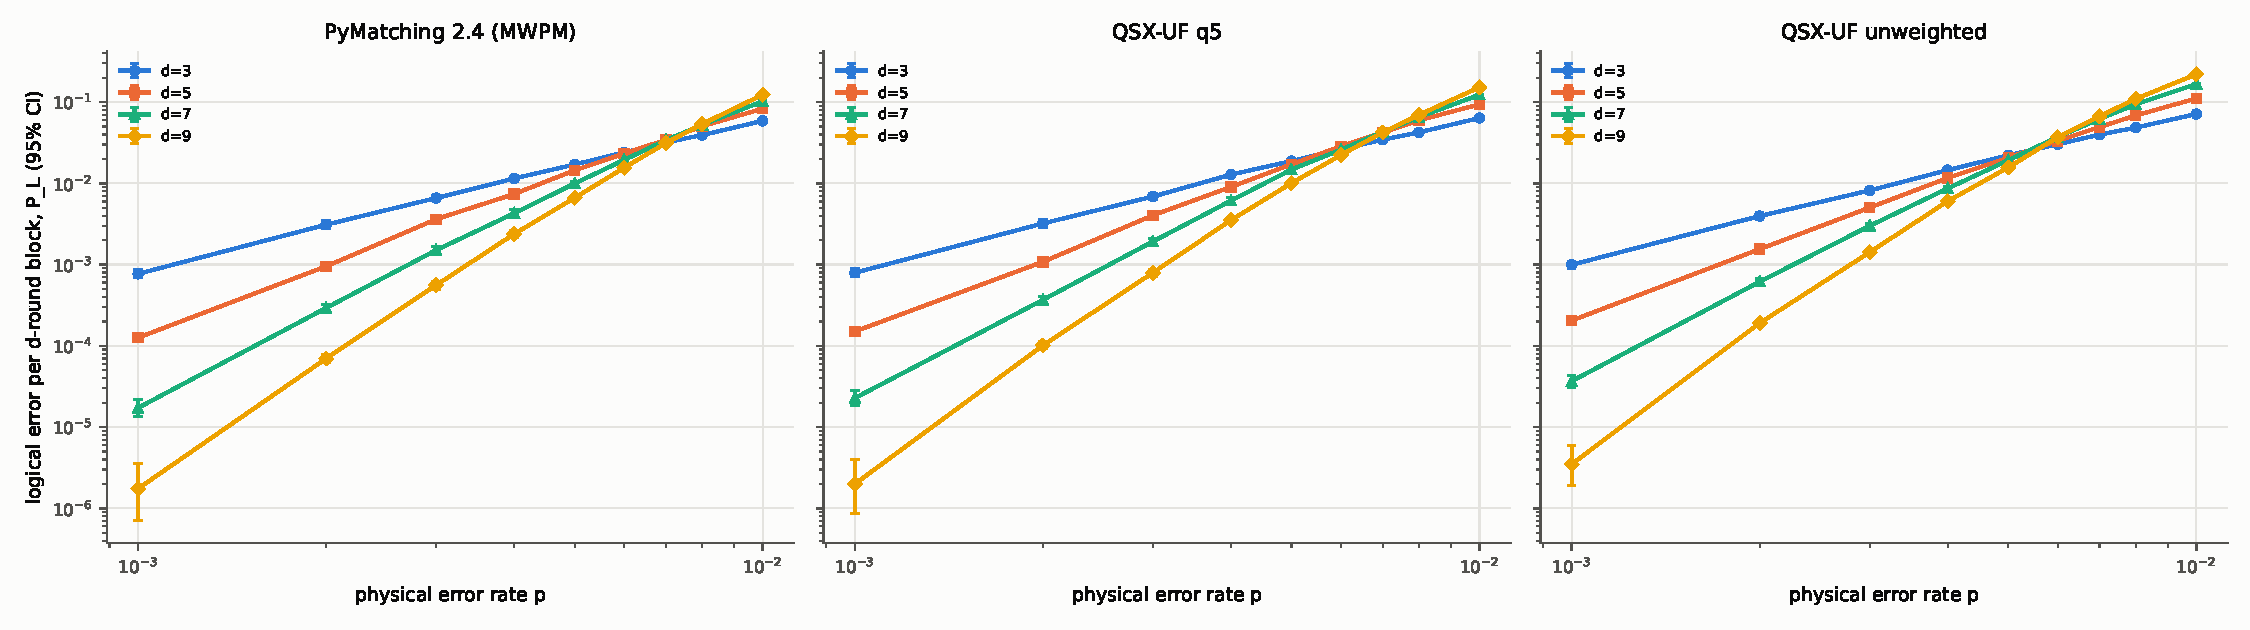
\includegraphics[width=\linewidth]{M1/figs/pl_vs_p.pdf}
\caption{P\textsubscript{L} vs.\ physical error rate (95\% CIs), circuit-level depolarizing noise, $d$ rounds.}
\label{fig:pl}
\end{figure}

\subsection{RTL correctness: co-simulation}
% AUTO-GENERATED by bench/claims_ext.py -- do not edit
\begin{table}[t]\centering\small
\caption{Co-simulation of the final RTL against the C++ golden model (status, rounds, observable, full correction bitmap and cycle count compared per syndrome). Columns: syndromes / mismatches.}
\label{tab:cosim}
\begin{tabular}{lrrrrrr}\toprule & \multicolumn{2}{c}{$d=3$} & \multicolumn{2}{c}{$d=5$} & \multicolumn{2}{c}{$d=7$} \\ \midrule
\claim{M2_ct_corerandom_lab} & \claim{M2_ct_corerandom_d3_sy} & \claim{M2_ct_corerandom_d3_mi} & \claim{M2_ct_corerandom_d5_sy} & \claim{M2_ct_corerandom_d5_mi} & \claim{M2_ct_corerandom_d7_sy} & \claim{M2_ct_corerandom_d7_mi} \\
\claim{M2_ct_corestim_lab} & \claim{M2_ct_corestim_d3_sy} & \claim{M2_ct_corestim_d3_mi} & \claim{M2_ct_corestim_d5_sy} & \claim{M2_ct_corestim_d5_mi} & \claim{M2_ct_corestim_d7_sy} & \claim{M2_ct_corestim_d7_mi} \\
\claim{M2_ct_sweep_lab} & \claim{M2_ct_sweep_d3_sy} & \claim{M2_ct_sweep_d3_mi} & \claim{M2_ct_sweep_d5_sy} & \claim{M2_ct_sweep_d5_mi} & \claim{M2_ct_sweep_d7_sy} & \claim{M2_ct_sweep_d7_mi} \\
\claim{M2_ct_toprandomstress_lab} & \claim{M2_ct_toprandomstress_d3_sy} & \claim{M2_ct_toprandomstress_d3_mi} & \claim{M2_ct_toprandomstress_d5_sy} & \claim{M2_ct_toprandomstress_d5_mi} & \claim{M2_ct_toprandomstress_d7_sy} & \claim{M2_ct_toprandomstress_d7_mi} \\
\claim{M2_ct_topstimstress_lab} & \claim{M2_ct_topstimstress_d3_sy} & \claim{M2_ct_topstimstress_d3_mi} & \claim{M2_ct_topstimstress_d5_sy} & \claim{M2_ct_topstimstress_d5_mi} & \claim{M2_ct_topstimstress_d7_sy} & \claim{M2_ct_topstimstress_d7_mi} \\
\bottomrule\end{tabular}\end{table}

Table~\ref{tab:cosim} summarises the campaign on the final RTL: \claim{M2_cosim_total} syndromes, with
\claim{M2_cosim_mm} mismatches in status, round count, observable, full correction bitmap or cycle count. The
shell runs inject malformed frames and incomplete configuration sessions. Every malformed frame was answered with
\texttt{FRAME\_ERROR} and every frame after an incomplete session with \texttt{CFG\_INVALID}, in order, as the
model predicts.

\subsection{Hardware: cycles, resources and latency}\label{sec:eval-hw}
TODO-hw

\subsection{Cost of the verified mechanisms}
Table~\ref{tab:overhead} separates the decoder core from the verified shell with a hierarchical synthesis
\stage{synth}. The shell contains the commit-on-last frame FIFO (backpressure, I1/P3), the atomic configuration
session with its written-word bitmap and range check (P5/P6), and the dispatcher, round-tag path and status gating
(P1--P4). At $d=5$ it costs \claim{M3_shell_lut_d5} LUT4 against \claim{M3_core_lut_d5} for the core
(\claim{M3_shell_lut_pct_d5}\%), but \claim{M3_shell_ff_pct_d5}\% of the flip-flops. Most of those FFs hold the
threshold table, which any configurable decoder needs; the atomicity bookkeeping itself is one bit per configuration
word plus one range-error bit. In time, framing and the handshakes add \claim{M3_shell_cycles_d3},
\claim{M3_shell_cycles_d5} and \claim{M3_shell_cycles_d7} cycles per frame at $d=3,5,7$ \stage{sim}: the input
header and syndrome beats, the dispatcher's load and the output header. Formal-only logic sits under
\texttt{ifdef FORMAL} and is not synthesised.
% AUTO-GENERATED by bench/claims_ext.py -- do not edit
\begin{table}[t]\centering\small
\caption{Core vs.\ verified shell (Yosys \texttt{synth\_ecp5 -noflatten}, LANES=8) and the shell's framing/handshake cycles per frame (Verilator, one frame in flight).}
\label{tab:overhead}
\begin{tabular}{lrrrrrrrr}\toprule & \multicolumn{3}{c}{core} & \multicolumn{3}{c}{shell} & & \\ & LUT4 & FF & BRAM & LUT4 & FF & BRAM & shell LUT & cycles \\ \midrule
$d=3$ & \claim{M3_core_lut_d3} & \claim{M3_core_ff_d3} & \claim{M3_core_bram_d3} & \claim{M3_shell_lut_d3} & \claim{M3_shell_ff_d3} & \claim{M3_shell_bram_d3} & \claim{M3_shell_lut_pct_d3}\% & \claim{M3_shell_cycles_d3} \\
$d=5$ & \claim{M3_core_lut_d5} & \claim{M3_core_ff_d5} & \claim{M3_core_bram_d5} & \claim{M3_shell_lut_d5} & \claim{M3_shell_ff_d5} & \claim{M3_shell_bram_d5} & \claim{M3_shell_lut_pct_d5}\% & \claim{M3_shell_cycles_d5} \\
\bottomrule\end{tabular}\end{table}


\subsection{WebAssembly runtime and the V8 patch}\label{sec:eval-wasm}
TODO-wasm

\subsection{Extensions}\label{sec:ext}
TODO-ext


\section{Threats to validity and limitations}\label{sec:limits}
\begin{itemize}
\item \textbf{No board.} Latency is cycles from a model that is cycle-exact with the RTL, divided by the
  post-PnR Fmax of one seed. Host--FPGA transport, clock-domain crossings and on-board jitter are not
  included. Energy is a toggle-count proxy, not Watts.
\item \textbf{Proof scope.} k-induction of the real core is for $d=3$ only. Larger cores are covered by
  co-simulation and one-step Z3 equivalence, which is not a proof of end-to-end equivalence. The TLA+ model is
  checked for small constants (stated in Table~\ref{tab:formal}). No proof says anything about
  P\textsubscript{L}.
\item \textbf{Noise model.} Uniform circuit-level depolarizing noise, memory experiments only, decoder
  graph built for the true $p$ (except in the noise-shift study). Real devices have leakage, crosstalk and
  non-uniform rates.
\item \textbf{CPU baselines.} One thread, batch-1 latency, timer resolution \claim{ENV_timer_ns}\,ns. The
  CPU numbers exclude syndrome acquisition, just as the hardware numbers exclude transport.
\item \textbf{Federated study.} A single-process simulation. The secure-aggregation masks assume no dropouts and
  honest-but-curious parties. The DP guarantee is per site, at record level, for the stated $(\varepsilon,\delta)$.
\end{itemize}

\section{Related work}
Union-find decoding was introduced by Delfosse and Nickerson \cite{delfosse2021uf} and extended to weighted
graphs \cite{huang2020weighted}. AFS \cite{das2022afs} proposed a UF-based hardware decoder architecture.
Helios \cite{liyanage2023helios} implemented a distributed UF decoder on FPGA, and Barber et
al.\ \cite{barber2023realtime} reported a real-time collision-clustering decoder on FPGA and ASIC. Software
MWPM via sparse blossom \cite{higgott2023sparse} in PyMatching \cite{higgott2022pymatching} is our baseline.
Neural decoders range from GNNs \cite{lange2023gnn} to transformer-based models trained on hardware data
\cite{bausch2024alphaqubit}. Our GNN is a small baseline, not a competitor to these. On the systems side, we
use TLA+ \cite{lamport2002tla}, Yosys/nextpnr \cite{shah2019nextpnr} and Z3 \cite{demoura2008z3}. We use FedAvg
\cite{mcmahan2017fedavg}, DP-SGD \cite{abadi2016dpsgd} with R\'enyi accounting \cite{mironov2017rdp,yousefpour2021opacus},
pairwise-mask secure aggregation \cite{bonawitz2017secagg} and Ed25519 \cite{bernstein2012ed25519}. What we
believe is new is the combination: a UF variant designed for bit-exact co-simulation, with its shell and host
protocol verified to stated bounds, and evaluated end to end with open tools.

\section{Conclusion}
TODO-conclusion

\bibliographystyle{plain}
\bibliography{refs}
\end{document}
